% 矩阵方程（一）：Sylvester方程AX+XB=C（线性算子表示与向量化、可解性与谱分离条件、Schur分解法、特征基下的求解）

\section{Sylvester方程}
\label{sec:ls-matrix-equations}

本节研究未知矩阵同时受左乘和右乘的Sylvester方程。先说明它是矩阵空间上的线性方程，再由两侧系数的特征值给出存在唯一性条件；计算时用正交Schur变换把方程化为准三角形后逐块回代，可对角化的系数还可以换到特征基逐元素相除。两条计算路线都不形成巨大的Kronecker系数矩阵。

\subsection{矩阵方程的线性算子表示}
\label{sec:ls-matrix-equation-types}

已知矩阵从左边、右边或两边作用在未知矩阵上，这样的方程称为\term{矩阵方程}（matrix equation）。最简单的是单侧方程$\bm A\bm X=\bm C$：$\bm X$的每一列分别满足一个以$\bm A$为系数的线性方程，所以它就是共用系数的多右端线性方程。双侧方程$\bm A\bm X\bm B=\bm C$中，$\bm A$作用在$\bm X$的列上，$\bm B$作用在$\bm X$的行上；两侧系数可逆时，可以先左乘$\bm A^{-1}$、再右乘$\bm B^{-1}$，两次“除法”互不干扰。

本节研究左右两种作用相加的\term{Sylvester方程}（Sylvester equation）
\begin{equation}
 \bm A\bm X+\bm X\bm B=\bm C,
 \label{eq:ls-sylvester-equation}
\end{equation}
其中$\bm A\in\mathbb R^{m\times m}$、$\bm B\in\mathbb R^{d\times d}$、$\bm C\in\mathbb R^{m\times d}$，未知量$\bm X\in\mathbb R^{m\times d}$。$\bm A$作用在$\bm X$的列上，阶数等于$\bm X$的行数；$\bm B$作用在$\bm X$的行上，阶数等于$\bm X$的列数。

两项相加以后，就不能分别“除以”两个系数。即使$\bm A$可逆，左乘$\bm A^{-1}$也只得到$\bm X+\bm A^{-1}\bm X\bm B=\bm A^{-1}\bm C$，未知量仍同时出现在两项中。所以必须把左边整体看作一个作用在$\bm X$上的映射。

记$\mathcal L(\bm X)=\bm A\bm X+\bm X\bm B$。由矩阵乘法的分配律，$\mathcal L$对$\bm X$是线性的，所以Sylvester方程就是$md$维空间$\mathbb R^{m\times d}$上的线性方程$\mathcal L(\bm X)=\bm C$。

为了写出它的系数矩阵，把矩阵按列拉直，并使用第~\ref{sec:ls-kronecker-products}节的恒等式
\[
 \operatorname{vec}(\bm A\bm X\bm B)=(\bm B^\top\otimes\bm A)\operatorname{vec}\bm X .
\]
把$\bm A\bm X$看成$\bm A\bm X\bm I_d$、把$\bm X\bm B$看成$\bm I_m\bm X\bm B$，相加得
\begin{equation}
 (\bm I_d\otimes\bm A+\bm B^\top\otimes\bm I_m)\operatorname{vec}\bm X
 =\operatorname{vec}\bm C .
 \label{eq:ls-sylvester-vectorized}
\end{equation}

记系数矩阵为$\bm K\in\mathbb R^{md\times md}$。这一表达说明，前面关于线性方程的判据都适用于Sylvester方程；对小例子，也可以直接用LU分解（第~\ref{sec:ls-lu}节）求解式~\eqref{eq:ls-sylvester-vectorized}来核验。但$\bm K$有$(md)^2$个元素，$m=d=100$时已达$10^8$个，稠密消元约需$\tfrac23(md)^3$次运算。所以向量化只用来理解线性结构和判断可解性，大规模求解应保留矩阵形状。

\subsection{可解性与唯一性条件}
\label{sec:ls-matrix-equation-existence}

单侧方程可以直接沿用列空间判据：$\bm A\bm X=\bm C$相容，当且仅当$\bm C$的每一列都在$\operatorname{range}(\bm A)$中，即$\operatorname{rank}[\bm A\ \bm C]=\operatorname{rank}(\bm A)$。双侧方程的相容性由向量化方程$(\bm B^\top\otimes\bm A)\operatorname{vec}\bm X=\operatorname{vec}\bm C$的增广秩判据判断。两侧系数都可逆时，唯一解为$\bm X=\bm A^{-1}\bm C\bm B^{-1}$；任一侧秩亏时，方程可能无解，有解时解也可以沿该侧的零空间变动，因而不唯一。

Sylvester方程不能这样逐侧处理，对角情形能看出原因。设$\bm A=\operatorname{diag}(\lambda_1,\ldots,\lambda_m)$、$\bm B=\operatorname{diag}(\mu_1,\ldots,\mu_d)$，则$\bm A\bm X$把第$i$行乘以$\lambda_i$，$\bm X\bm B$把第$j$列乘以$\mu_j$。于是方程按元素分解为
\[
 (\lambda_i+\mu_j)\,x_{i,j}=c_{i,j},
\]
分母非零时
\begin{equation}
 x_{i,j}=\frac{c_{i,j}}{\lambda_i+\mu_j}.
 \label{eq:ls-sylvester-diagonal-closed-form}
\end{equation}

若某个$\lambda_i+\mu_j=0$，该位置退化为$0\cdot x_{i,j}=c_{i,j}$：$c_{i,j}\neq0$时无解，$c_{i,j}=0$时$x_{i,j}$可以任取。所以决定可解性的，是$\bm A$的特征值与$-\bm B$的特征值是否重合（图~\ref{fig:ls-sylvester-separation}），而不是两侧系数各自是否可逆。一般情形的结论相同，只是实矩阵的特征值可能是复数，条件要在复数域中检查。下面记$\operatorname{spec}(\bm A)$为$\bm A$在复数域中的全体特征值。

\begin{figure}[htbp]
  \centering
  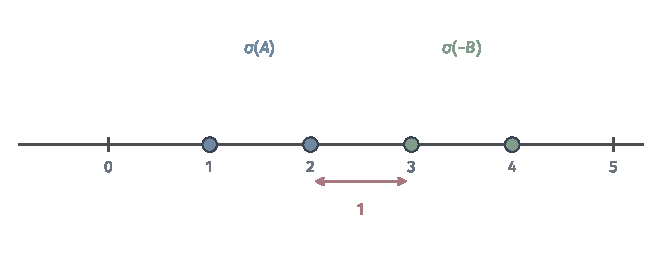
\includegraphics[width=112mm]{figures/00-shared/mathematical-preliminaries-upper/02-linear-spaces/matplotlib/ls-sylvester-separation/ls-sylvester-separation.pdf}
  \caption{谱分离条件的实轴示意。$\bm A=\operatorname{diag}(1,2)$的特征值$\{1,2\}$与$-\bm B$（$\bm B=\operatorname{diag}(-3,-4)$）的特征值$\{3,4\}$不相交，最近一对相距$1$，所以四个分母$\lambda_i+\mu_j$都不为零，对任意$\bm C$方程都有唯一解。}
  \label{fig:ls-sylvester-separation}
\end{figure}

\begin{theorem}[Sylvester方程的唯一可解性]
\label{thm:ls-sylvester-unique-solvability}
设$\bm A\in\mathbb R^{m\times m}$、$\bm B\in\mathbb R^{d\times d}$。方程$\bm A\bm X+\bm X\bm B=\bm C$对每个$\bm C\in\mathbb R^{m\times d}$都有唯一解，当且仅当
\begin{equation}
 \operatorname{spec}(\bm A)\cap\operatorname{spec}(-\bm B)=\varnothing ,
 \label{eq:ls-sylvester-spectral-separation}
\end{equation}
即对$\bm A$的任一特征值$\lambda$与$\bm B$的任一特征值$\mu$，都有$\lambda+\mu\neq0$。
\end{theorem}

\begin{proof}
$\mathcal L$把$\mathbb R^{m\times d}$映到自身。由秩零度定理，它对每个右端唯一可解，当且仅当齐次方程只有零解，也就是$\det\bm K\neq0$。这个行列式在实数域和复数域中是同一个数，所以可以在复数域中讨论齐次方程。

必要性。设$\bm A\bm u=\lambda\bm u$，且$-\lambda$是$\bm B$的特征值。$\bm B^\top$与$\bm B$有相同的特征多项式，所以$-\lambda$也是$\bm B^\top$的特征值，可取$\bm B^\top\bm w=-\lambda\bm w$，其中$\bm u,\bm w\neq\bm0$。于是$\bm X=\bm u\bm w^\top\neq\bm0$满足
\[
 \bm A\bm X+\bm X\bm B=\lambda\bm u\bm w^\top+\bm u(\bm B^\top\bm w)^\top=\lambda\bm u\bm w^\top-\lambda\bm u\bm w^\top=\bm0 ,
\]
齐次方程有非零解。

充分性。设$\bm A\bm X+\bm X\bm B=\bm0$，即$\bm A\bm X=\bm X(-\bm B)$。归纳得$\bm A^k\bm X=\bm X(-\bm B)^k$，从而对任意多项式$p$有
\[
 p(\bm A)\bm X=\bm X\,p(-\bm B) .
\]
取$p(z)=\prod_k(z-\lambda_k)$为$\bm A$的特征多项式，由Cayley--Hamilton定理~\ref{thm:ls-cayley-hamilton}，$p(\bm A)=\bm0$。另一方面，$p(-\bm B)=\prod_k(-\bm B-\lambda_k\bm I)$中每个$\lambda_k$都不是$-\bm B$的特征值，各因子可逆，所以$p(-\bm B)$可逆。于是$\bm X\,p(-\bm B)=\bm0$推出$\bm X=\bm0$。
\end{proof}

这一条件与$\bm A$、$\bm B$各自是否可逆无关。$\bm A=\bm0$、$\bm B=\bm I_d$时$\bm A$不可逆，方程却化为$\bm X=\bm C$，唯一可解；$1\times1$情形$\bm A=2$、$\bm B=-2$都可逆，方程却是$0\cdot x=c$。

谱不相交只回答解是否唯一，不回答解对数据误差是否敏感。对角情形下，最小的$|\lambda_i+\mu_j|$越接近零，$\bm C$的误差被放大得越多；矩阵远离正规时，即使所有谱和都远离零，解仍可能很敏感，第~\ref{sec:ls-sylvester-diagonalizable}节会看到其中的原因。

\subsection{Schur分解法}
\label{sec:ls-sylvester-schur}

稠密的一般Sylvester方程通常用\term{Bartels--Stewart算法}（Bartels--Stewart algorithm）求解。它的思路与解三角方程组相同：先用正交相似把两个系数化为准上三角形，未知元之间就有了先后依赖，可以逐个回代。下面设谱条件~\eqref{eq:ls-sylvester-spectral-separation}成立，依次说明变换、回代次序和二阶块的处理，再给出算法步骤、算例与分析。

\paragraph{主要思想：正交变换到准三角形}
第一步，分别对两个系数作实Schur分解（定理~\ref{thm:ls-real-schur}）
\[
 \bm A=\bm U\bm T\bm U^\top,\qquad \bm B=\bm V\bm S\bm V^\top,
\]
其中$\bm U,\bm V$正交，$\bm T,\bm S$是准上三角矩阵，对角块为$1\times1$（实特征值）或$2\times2$（一对共轭复特征值）。这一步只依赖$\bm A$、$\bm B$，与右端无关。

把分解代入$\bm A\bm X+\bm X\bm B=\bm C$，得
\[
 \bm U\bm T\bm U^\top\bm X+\bm X\bm V\bm S\bm V^\top=\bm C .
\]
两边左乘$\bm U^\top$、右乘$\bm V$，利用$\bm U^\top\bm U=\bm I$、$\bm V^\top\bm V=\bm I$，并记$\bm Y=\bm U^\top\bm X\bm V$、$\bm D=\bm U^\top\bm C\bm V$，方程化为
\begin{equation}
 \bm T\bm Y+\bm Y\bm S=\bm D .
 \label{eq:ls-sylvester-transformed}
\end{equation}
$\bm T$与$\bm A$、$\bm S$与$\bm B$分别相似，特征值相同，所以新方程同样满足谱条件。正交变换还不改变Frobenius范数：任一近似解$\bm Z$在原坐标中的残差，等于$\bm W=\bm U^\top\bm Z\bm V$在新坐标中的残差（下面定理~\ref{thm:ls-bartels-stewart}的第三条）。因此在新坐标中解得准确，换回原坐标后残差不会被放大。

\paragraph{主要思想：上三角情形的回代次序}
先看$\bm T$、$\bm S$都是上三角的情形。比较式~\eqref{eq:ls-sylvester-transformed}两边的$(i,j)$元，其中
\[
 (\bm T\bm Y)_{i,j}=\sum_{k\geq i}t_{i,k}y_{k,j},\qquad
 (\bm Y\bm S)_{i,j}=\sum_{\ell\leq j}y_{i,\ell}s_{\ell,j}.
\]
把含$y_{i,j}$的两项留在左边，得
\begin{equation}
 (t_{i,i}+s_{j,j})\,y_{i,j}
 =d_{i,j}-\sum_{k>i}t_{i,k}y_{k,j}-\sum_{\ell<j}y_{i,\ell}s_{\ell,j}.
 \label{eq:ls-sylvester-triangular-entry}
\end{equation}
右端第一个和只用同一列中更靠下的元素，第二个和只用同一行中更靠左的元素。所以按列$j=1,\ldots,d$从左向右，每列内按行$i=m,\ldots,1$从下向上计算，每一步右端都已知。除数$t_{i,i}+s_{j,j}$是$\bm A$与$\bm B$的一对特征值之和，由谱条件不为零。

同一次序也可以按整列写出。$\bm Y\bm S$的第$j$列是$\sum_{\ell\leq j}s_{\ell,j}\bm y_\ell$，比较式~\eqref{eq:ls-sylvester-transformed}两边的第$j$列，得
\begin{equation}
 (\bm T+s_{j,j}\bm I_m)\bm y_j=\bm d_j-\sum_{\ell<j}s_{\ell,j}\bm y_\ell .
 \label{eq:ls-sylvester-column-recursion}
\end{equation}
右端只用到更靠左的列；每列的系数是上三角矩阵，用第~\ref{sec:ls-lu}节的回代从最后一行向上求解，逐行展开正是式~\eqref{eq:ls-sylvester-triangular-entry}。图~\ref{fig:ls-bartels-stewart-column-order}画出了第$j$列的依赖：$\bm S$第$j$列中对角线以上的元素把已求出的列带进右端，对角元$s_{j,j}$并入当前列的三角系数。

\begin{figure}[htbp]
  \centering
  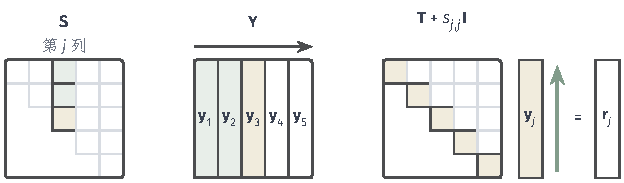
\includegraphics[width=109.6mm]{figures/01-basic-mathematics/03-vectors-matrices-and-multivariate-functions/tikz/c5-bartels-stewart-column-order/figure.pdf}
  \caption{Bartels--Stewart算法逐列求解$\bm T\bm Y+\bm Y\bm S=\bm D$的次序（上三角情形，图中取当前列$j=3$）。左：$\bm S$的第$j$列，绿色元素$s_{\ell,j}$（$\ell<j$）对应已求出的列，黄色为$s_{j,j}$。中：$\bm Y$的列从左到右求出。右：当前列解一个对角元为$t_{i,i}+s_{j,j}$的上三角方程组，从最后一行向上回代。}
  \label{fig:ls-bartels-stewart-column-order}
\end{figure}

\paragraph{主要思想：二阶对角块的局部系统}
实Schur形含$2\times2$对角块时，把一个标量未知数换成一个未知子块。按$\bm T$、$\bm S$的对角块把$\bm Y$、$\bm D$分块，记$\bm T$的第$I$个对角块为$\bm T_{I,I}$、$\bm S$的第$J$个对角块为$\bm S_{J,J}$，比较第$(I,J)$块得
\begin{equation}
 \begin{aligned}
 \bm T_{I,I}\bm Y_{I,J}+\bm Y_{I,J}\bm S_{J,J}
 &=\bm D_{I,J}-\sum_{K>I}\bm T_{I,K}\bm Y_{K,J}\\
 &\quad-\sum_{L<J}\bm Y_{I,L}\bm S_{L,J}.
 \end{aligned}
 \label{eq:ls-sylvester-block-recursion}
\end{equation}
右端只含同一块列中更靠下的块和更靠左的块列，因此按块列从左到右、每块列从下到上计算。

左边是一个小Sylvester方程，$\bm Y_{I,J}$至多是$2\times2$的，至多含四个未知数。由式~\eqref{eq:ls-sylvester-vectorized}，它的向量化系数是$\bm I\otimes\bm T_{I,I}+\bm S_{J,J}^\top\otimes\bm I$，至多为$4$阶，直接消元即可；只在这样的局部形成Kronecker系数。$\bm T_{I,I}$的特征值是$\bm A$的特征值，$\bm S_{J,J}$的特征值是$\bm B$的特征值，所以局部方程满足谱条件，由定理~\ref{thm:ls-sylvester-unique-solvability}唯一可解。

\paragraph{算法实现}
把上面三步连起来，Bartels--Stewart算法如下。
\begin{enumerate}
 \item 计算实Schur分解$\bm A=\bm U\bm T\bm U^\top$、$\bm B=\bm V\bm S\bm V^\top$，并变换右端$\bm D=\bm U^\top\bm C\bm V$。
 \item 按块列从左到右、每块列从下到上的次序，对每个块$(I,J)$从$\bm D_{I,J}$中减去已求出块的贡献，再解至多四个未知数的局部方程，得$\bm Y_{I,J}$。
 \item 恢复原未知量$\bm X=\bm U\bm Y\bm V^\top$，并在原方程中计算残差$\bm A\bm X+\bm X\bm B-\bm C$。精确算术下它为零；浮点计算中它的Frobenius范数与新坐标中的残差相同，可以直接用来检验整个流程。
\end{enumerate}
局部方程的系数接近奇异时，除法会放大误差，中间量也可能溢出。数值软件库中的实现因此常引入一个缩放因子$\sigma\in(0,1]$，实际求解$\bm T\bm Y+\bm Y\bm S=\sigma\bm D$，再连同$\sigma$一起返回，并对过小的局部分母给出警告。使用者应把$\sigma<1$或这类警告视为方程接近不可解的信号，而不是忽略它。

\begin{example}[Schur形方程的逐元素回代]
\label{ex:ls-sylvester-schur-form-entries}
先跳过Schur分解，直接从已为Schur形的系数出发，看逐元素回代应按什么次序进行。两个系数取为上三角矩阵
\[
 \bm T=\begin{bmatrix}1&2\\0&3\end{bmatrix},\qquad
 \bm S=\begin{bmatrix}4&1\\0&5\end{bmatrix},
\]
右端取为
\[
 \bm D=\begin{bmatrix}11&21\\21&35\end{bmatrix}.
\]
谱和$t_{i,i}+s_{j,j}$为$5,6,7,8$，都不为零，每个局部方程都可以相除。按式~\eqref{eq:ls-sylvester-triangular-entry}，第$1$列从下向上：
\[
 y_{2,1}=\frac{21}{3+4}=3,\qquad
 y_{1,1}=\frac{11-t_{1,2}y_{2,1}}{1+4}=\frac{11-2\cdot3}{5}=1 .
\]
第$2$列从下向上，右端还要减去左边一列经$s_{1,2}=1$带来的贡献：
\[
 \begin{aligned}
 y_{2,2}&=\frac{35-y_{2,1}s_{1,2}}{3+5}=\frac{35-3}{8}=4,\\
 y_{1,2}&=\frac{21-t_{1,2}y_{2,2}-y_{1,1}s_{1,2}}{1+5}=\frac{21-8-1}{6}=2 .
 \end{aligned}
\]
于是
\[
 \bm Y=\begin{bmatrix}1&2\\3&4\end{bmatrix}.
\]

代回检查全部四个元素：
\[
 \bm T\bm Y+\bm Y\bm S
 =\begin{bmatrix}7&10\\9&12\end{bmatrix}+\begin{bmatrix}4&11\\12&23\end{bmatrix}
 =\begin{bmatrix}11&21\\21&35\end{bmatrix}=\bm D .
\]
若次序颠倒，例如先算$y_{1,1}$，它的右端需要尚未求出的$y_{2,1}$，回代无法进行。
\end{example}

上例跳过了Schur分解。下面的例子从一般系数出发，完整走一遍变换、回代和恢复。

\begin{example}[Bartels--Stewart求解一个二阶方程]
\label{ex:ls-bartels-stewart-2x2}
系数取为
\[
 \bm A=\begin{bmatrix}-2&3\\-4&5\end{bmatrix},\qquad
 \bm B=\begin{bmatrix}1&1\\0&3\end{bmatrix},
\]
右端取为
\[
 \bm C=\begin{bmatrix}1&12\\-2&21\end{bmatrix}.
\]
$\bm A$的特征值为$2,1$，$-\bm B$的特征值为$-1,-3$，谱条件成立。

先作实Schur分解。由$\bm A(3,4)^\top=2(3,4)^\top$取
\[
 \bm U=\frac15\begin{bmatrix}3&-4\\4&3\end{bmatrix},\qquad
 \bm T=\bm U^\top\bm A\bm U=\begin{bmatrix}2&7\\0&1\end{bmatrix};
\]
$\bm B$已是上三角，取$\bm V=\bm I$、$\bm S=\bm B$。变换右端得
\[
 \bm D=\bm U^\top\bm C=\begin{bmatrix}-1&24\\-2&3\end{bmatrix}.
\]

在Schur坐标下逐列求解。第$1$列解$(\bm T+s_{1,1}\bm I)\bm y_1=\bm d_1$，即
\[
 \begin{bmatrix}3&7\\0&2\end{bmatrix}\bm y_1=\begin{bmatrix}-1\\-2\end{bmatrix},
\]
从下往上得$y_{2,1}=-1$、$y_{1,1}=2$。第$2$列的右端为
\[
 \bm d_2-s_{1,2}\bm y_1=(24,3)^\top-(2,-1)^\top=(22,4)^\top ,
\]
解
\[
 \begin{bmatrix}5&7\\0&4\end{bmatrix}\bm y_2=\begin{bmatrix}22\\4\end{bmatrix}
\]
得$y_{2,2}=1$、$y_{1,2}=3$。

变回原坐标，
\[
 \bm X=\bm U\bm Y=\frac15\begin{bmatrix}3&-4\\4&3\end{bmatrix}\begin{bmatrix}2&3\\-1&1\end{bmatrix}=\begin{bmatrix}2&1\\1&3\end{bmatrix}.
\]
核验：
\[
 \bm A\bm X+\bm X\bm B
 =\begin{bmatrix}-1&7\\-3&11\end{bmatrix}+\begin{bmatrix}2&5\\1&10\end{bmatrix}
 =\begin{bmatrix}1&12\\-2&21\end{bmatrix}=\bm C ,
\]
原方程残差为零。
\end{example}

\paragraph{算法分析：正确性}
上面的推导说明每一步都能进行，而且按次序算出的块满足各自的块等式。把这些事实合在一起，就得到算法的正确性和残差检验的依据。

\begin{theorem}[Bartels--Stewart算法的正确性]
\label{thm:ls-bartels-stewart}
设$\bm A=\bm U\bm T\bm U^\top$、$\bm B=\bm V\bm S\bm V^\top$是实Schur分解，谱条件~\eqref{eq:ls-sylvester-spectral-separation}成立，$\bm D=\bm U^\top\bm C\bm V$。则
\begin{enumerate}
 \item 按块列从左到右、每块列从下到上的次序，每一步的局部方程$\bm T_{I,I}\bm Y_{I,J}+\bm Y_{I,J}\bm S_{J,J}=\bm E_{I,J}$都唯一可解，其中右端$\bm E_{I,J}$由已求出的块给出；
 \item 由此算出的$\bm Y$是方程~\eqref{eq:ls-sylvester-transformed}的唯一解，$\bm X=\bm U\bm Y\bm V^\top$是$\bm A\bm X+\bm X\bm B=\bm C$的唯一解；
 \item 对任意$\bm Z\in\mathbb R^{m\times d}$，记$\bm W=\bm U^\top\bm Z\bm V$，有$\lVert\bm A\bm Z+\bm Z\bm B-\bm C\rVert_{\mathrm F}=\lVert\bm T\bm W+\bm W\bm S-\bm D\rVert_{\mathrm F}$。
\end{enumerate}
\end{theorem}

\begin{proof}
先证第三条。由$\bm A=\bm U\bm T\bm U^\top$、$\bm B=\bm V\bm S\bm V^\top$与$\bm Z=\bm U\bm W\bm V^\top$，
\[
 \bm A\bm Z+\bm Z\bm B-\bm C=\bm U(\bm T\bm W+\bm W\bm S-\bm D)\bm V^\top,
\]
而左右乘正交矩阵不改变Frobenius范数。

再证第一条。准上三角矩阵的特征值是各对角块特征值的并，$\bm T$与$\bm A$相似，所以$\bm T_{I,I}$的特征值都是$\bm A$的特征值；同理$\bm S_{J,J}$的特征值都是$\bm B$的特征值。于是每个局部方程满足谱条件，由定理~\ref{thm:ls-sylvester-unique-solvability}唯一可解。

最后证第二条。第$(I,J)$块等式的右端只含按次序已算出的块，所以算出的每一块都满足相应的块等式；全部块等式合起来就是式~\eqref{eq:ls-sylvester-transformed}。$\bm T$、$\bm S$满足谱条件，由定理~\ref{thm:ls-sylvester-unique-solvability}，这个解唯一。在第三条中取$\bm Z=\bm X$、$\bm W=\bm Y$，得原方程残差为零；原方程的唯一性同样由该定理给出。
\end{proof}

\paragraph{算法分析：计算代价}
实Schur分解靠迭代算出，常用实现计入正交因子约需$25m^3$与$25d^3$次运算\scite{math-golub2013matrix}。变换右端与变回原坐标各约$2(m^2d+md^2)$次，逐块回代约$m^2d+md^2$次；存储只需$O(m^2+d^2+md)$个数。$m=d=100$时总量约$6\times10^7$次，而对式~\eqref{eq:ls-sylvester-vectorized}作稠密LU约需$7\times10^{11}$次，并要存储$10^8$个数。多组右端共用$\bm A$、$\bm B$时，两个Schur分解只做一次，每增加一个右端只增加$O(m^2d+md^2)$次运算。

\subsection{特征基下的求解}
\label{sec:ls-sylvester-diagonalizable}

当$\bm A$、$\bm B$都可对角化时，可以换到各自的特征基，把方程化为式~\eqref{eq:ls-sylvester-diagonal-closed-form}的对角情形。设$\bm A=\bm P\bm\Lambda\bm P^{-1}$、$\bm B=\bm R\bm M\bm R^{-1}$，其中$\bm\Lambda=\operatorname{diag}(\lambda_i)$、$\bm M=\operatorname{diag}(\mu_j)$。这条路线公式最简短，代价是换基矩阵一般不正交。

\paragraph{主要思想：换到特征基}
记$\bm Y=\bm P^{-1}\bm X\bm R$、$\bm D=\bm P^{-1}\bm C\bm R$。方程左乘$\bm P^{-1}$、右乘$\bm R$，由$\bm P^{-1}\bm A=\bm\Lambda\bm P^{-1}$与$\bm B\bm R=\bm R\bm M$化为
\[
 \bm\Lambda\bm Y+\bm Y\bm M=\bm D .
\]
这时各坐标完全解耦，逐元素得到
\[
 (\lambda_i+\mu_j)\,y_{i,j}=d_{i,j}.
\]
谱条件成立时所有分母非零，$y_{i,j}=d_{i,j}/(\lambda_i+\mu_j)$。若某个$\lambda_i+\mu_j=0$，就要区分两种情形：$d_{i,j}\neq0$时这个坐标无解，$d_{i,j}=0$时$y_{i,j}$是自由变量。注意检查的是变换后的$d_{i,j}$，而不是原右端的$c_{i,j}$。

\paragraph{主要思想：恢复原未知量}
恢复公式为$\bm X=\bm P\bm Y\bm R^{-1}$，次序与换基相反。与Schur路线不同，这里的换基矩阵$\bm P$、$\bm R$一般不正交：变换右端和还原解时，误差可能被放大$\kappa_2(\bm P)\kappa_2(\bm R)$量级，所以实现前要检查两组特征基的条件数（见下面的算法分析）。实矩阵有复特征值时，$\bm P$、$\bm R$为复矩阵，全程用复数运算，最后舍去舍入产生的虚部。

\paragraph{算法实现}
算法依次执行以下步骤。
\begin{enumerate}
 \item 核验两组特征基可逆且条件数可以接受；若特征基不满秩或接近奇异，改用第~\ref{sec:ls-sylvester-schur}节的Schur路线，不尝试直接求逆。
 \item 变换右端时不求逆：先对$\bm P$作LU分解，对$\bm C$的各列求解$\bm P\bm Z=\bm C$，再令$\bm D=\bm Z\bm R$。
 \item 逐项检查谱和$\lambda_i+\mu_j$并相除，得$\bm Y$。
 \item 先算$\bm W=\bm P\bm Y$，再利用$\bm R$的LU分解求解$\bm X\bm R=\bm W$，得$\bm X=\bm P\bm Y\bm R^{-1}$；最后在原方程中计算残差。
\end{enumerate}

\begin{example}[对角系数下的逐元素相除与零谱和]
\label{ex:ls-sylvester-diagonal-zero-sum}
下面用以下数据演示：
\[
 \bm A=\operatorname{diag}(1,2),\qquad \bm B=\operatorname{diag}(3,4),\qquad
 \bm C=\begin{bmatrix}4&10\\15&24\end{bmatrix}.
\]
两个系数都是对角矩阵，所以$\bm P=\bm R=\bm I$，$\bm D=\bm C$，四个谱和为$1+3=4$、$1+4=5$、$2+3=5$、$2+4=6$。逐元素相除得
\[
 x_{1,1}=\frac44=1,\quad x_{1,2}=\frac{10}5=2,\quad
 x_{2,1}=\frac{15}5=3,\quad x_{2,2}=\frac{24}6=4,
\]
即$\bm X=\bigl[\begin{smallmatrix}1&2\\3&4\end{smallmatrix}\bigr]$。四个元素互不耦合，每个只需一次除法。代回原方程，
\[
 \bm A\bm X+\bm X\bm B
 =\begin{bmatrix}1&2\\6&8\end{bmatrix}+\begin{bmatrix}3&8\\9&16\end{bmatrix}
 =\bm C .
\]

再把右下角的谱和改为零：令$\bm B=\operatorname{diag}(3,-2)$，则$\lambda_2+\mu_2=0$，其余三个谱和$4,-1,5$仍非零。第$(2,2)$个方程变为$0\cdot x_{2,2}=c_{2,2}$。右端保持$c_{2,2}=24\neq0$时，方程无解；把右端改为$c_{2,2}=0$时，$x_{1,1},x_{1,2},x_{2,1}$仍由各自的除法唯一确定，$x_{2,2}$可以任取，解集是一条直线。
\end{example}

对角系数无须换基。下面的例子换到非正交的特征基，再除以谱和、还原。

\begin{example}[特征基下的逐元素求解]
\label{ex:ls-sylvester-eigenbasis}
系数取为
\[
 \bm A=\begin{bmatrix}1&1\\0&2\end{bmatrix},\qquad
 \bm B=\begin{bmatrix}3&1\\0&4\end{bmatrix},
\]
右端取为
\[
 \bm C=\begin{bmatrix}7&12\\15&21\end{bmatrix}.
\]
两者的特征向量都是$(1,0)^\top$与$(1,1)^\top$，故$\bm P=\bm R=\bigl[\begin{smallmatrix}1&1\\0&1\end{smallmatrix}\bigr]$，特征值分别为$1,2$与$3,4$，四个分母$\lambda_i+\mu_j$为$4,5,5,6$。

先换基，变换后的右端为
\[
 \bm D=\bm P^{-1}\bm C\bm R=\begin{bmatrix}-8&-17\\15&36\end{bmatrix}.
\]
再逐元素除以谱和，得
\[
 \bm Y=\begin{bmatrix}-2&-17/5\\3&6\end{bmatrix}.
\]
最后变回原坐标，
\[
 \bm X=\bm P\bm Y\bm R^{-1}=\begin{bmatrix}1&8/5\\3&3\end{bmatrix}.
\]

代回原方程，
\[
 \bm A\bm X+\bm X\bm B
 =\begin{bmatrix}4&23/5\\6&6\end{bmatrix}+\begin{bmatrix}3&37/5\\9&15\end{bmatrix}
 =\bm C ,
\]
残差为零。

若把$\bm B$的$(1,1)$元改为$-2$，则$\mu_1=-2$，$\lambda_2+\mu_1=0$。这时$\bm B$的特征基也随之改变，第$(2,1)$个方程变为$0\cdot y_{2,1}=d_{2,1}$，其中$d_{2,1}$是按新的特征基变换后的右端：$d_{2,1}\neq0$时无解，$d_{2,1}=0$时解不唯一。
\end{example}

\paragraph{算法分析：数值敏感度}
这条路线只在特征基接近正交时可靠。记$\delta_{\min}=\min_{i,j}|\lambda_i+\mu_j|$，由逐元素相除得
\[
 \lVert\bm Y\rVert_{\mathrm F}\leq\frac{\lVert\bm D\rVert_{\mathrm F}}{\delta_{\min}} .
\]
再对$\bm D=\bm P^{-1}\bm C\bm R$与$\bm X=\bm P\bm Y\bm R^{-1}$使用不等式
\[
 \lVert\bm M_1\bm Z\bm M_2\rVert_{\mathrm F}\leq\lVert\bm M_1\rVert_2\lVert\bm Z\rVert_{\mathrm F}\lVert\bm M_2\rVert_2 ,
\]
只能得到

\begin{equation}
 \lVert\bm X\rVert_{\mathrm F}
 \leq\frac{\kappa_2(\bm P)\,\kappa_2(\bm R)}{\delta_{\min}}\lVert\bm C\rVert_{\mathrm F},
 \label{eq:ls-sylvester-eigenbasis-bound}
\end{equation}
所以在斜基下，谱和远离零并不独自保证良好条件。

换基本身也会放大误差：$\bm P^{-1}\bm C$的元素可以比$\bm C$大$\kappa_2(\bm P)$量级，变回时再相互抵消。例如$0<\epsilon\ll1$时，$\bm A=\bigl[\begin{smallmatrix}1&1\\0&1+\epsilon\end{smallmatrix}\bigr]$的特征向量$(1,0)^\top$与$(1,\epsilon)^\top$几乎平行，$\kappa_2(\bm P)\geq1/\epsilon$，中间量的大小约为$1/\epsilon$，舍入误差随之被放大。

$\bm A$、$\bm B$实对称时，谱定理~\ref{thm:ls-real-symmetric-spectral}给出正交特征基，$\kappa_2=1$，元素公式既简单又可靠。一般情形即使可以对角化，也宜使用第~\ref{sec:ls-sylvester-schur}节的正交Schur变换。
